% ICASSP 2027 draft using the official 2027 author-kit layout.
\RequirePackage{fix-cm}
\documentclass{article}

\usepackage{spconf,amsmath,amssymb,upgreek,graphicx,booktabs,array,xcolor}
\usepackage{xurl}
\usepackage{microtype}
\usepackage{flushend}

\urlstyle{same}
\raggedbottom

% Review-only emphasis. Change to \reviewchangesfalse for the submission PDF.
\newif\ifreviewchanges
\reviewchangesfalse
\newcommand{\edited}[1]{#1}
\newcommand{\corrected}[1]{{\ifreviewchanges\bfseries\boldmath\fi #1}}

\setlength{\textfloatsep}{6pt plus 2pt minus 2pt}
\setlength{\dbltextfloatsep}{6pt plus 2pt minus 2pt}
\setlength{\floatsep}{5pt plus 2pt minus 1pt}
\setlength{\dblfloatsep}{5pt plus 2pt minus 1pt}
\setlength{\intextsep}{6pt plus 2pt minus 2pt}
\setlength{\abovecaptionskip}{2pt}
\setlength{\belowcaptionskip}{2pt}
\setlength{\smallskipamount}{1pt plus .5pt minus .5pt}

\makeatletter
\renewcommand\normalsize{\@setfontsize\normalsize{9.5pt}{11.4pt}}
\normalsize
% Keep the paper-kit title spacing while avoiding spconf's redundant blank row
% between \name and \address.
\renewcommand{\name}[1]{\gdef\@name{{\em #1}}}
\def\@maketitle{\newpage
 \null
 \vskip 2em \begin{center}
 {\large \bf \@title \par} \vskip 1.5em {\large \lineskip .5em
\begin{tabular}[t]{c}\@name \\ \@address
 \end{tabular}\par} \end{center}
 \par
 \vskip 1.5em}
\renewcommand\section{\@startsection{section}{1}{\z@}%
  {-2.5ex plus -.5ex minus -.2ex}{1ex plus .2ex}{\normalfont\normalsize\bfseries\centering}}
\renewcommand\subsection{\@startsection{subsection}{2}{\z@}%
  {-2ex plus -.4ex minus -.2ex}{.8ex plus .2ex}{\normalfont\normalsize\bfseries}}
\let\standardthebibliography\thebibliography
\renewcommand{\thebibliography}[1]{%
  \standardthebibliography{#1}%
  \small
  \setlength{\itemsep}{9pt}%
  \setlength{\parsep}{0pt}%
}
\makeatother

\newcommand{\tauvoice}{$\uptau$-Voice}
\newcommand{\passone}{\mbox{Pass@1}}
\newcommand{\passk}{$\mathrm{Pass}^{3}$}
\newcommand{\telicit}{$\uptau$-Elicitation}

\title{TAU-ELICITATION: BENCHMARKING MULTI-TURN ENTITY EXTRACTION IN VOICE AGENTS}

\name{Soham Ray$^{1}$ \qquad Victor Barres$^{2}$}
\address{$^{1}$Sierra \qquad $^{2}$Mercor}

\begin{document}

\maketitle

\begin{abstract}
Voice agents often need to collect names, addresses, identifiers, dates, and
times exactly, yet end-to-end benchmarks obscure where capture fails. We
introduce \telicit{}, a 200-task voice benchmark spanning 10 entity types,
controlled difficulty, caller realisms, and three environments. \edited{A text
control} passes all tasks, but four voice configurations achieve robust exact
success on only \corrected{14--45\%}. Agents increase verification for hard and
unfamiliar entities and sometimes for incorrect captures, \corrected{yet only
30--37\% of verified errors are repaired}.
\edited{Scaffolded runs have robust \passk{} scores \corrected{13--30} percentage
points higher and take 21--28 seconds longer per call.}
Realisms such as spelling variations and restarts do not detectably affect
exact success; mispronunciation increases repair effort. These results
\edited{suggest that strategy selection and successful recovery are key bottlenecks}
in exact spoken entity collection.
\end{abstract}

\begin{keywords}
voice agents, spoken dialogue evaluation, multi-turn entity extraction,
conversational repair, task-oriented dialogue
\end{keywords}

\section{Introduction}
\label{sec:introduction}

Voice-agent benchmarks usually score complete tasks
\cite{ray2026tauvoice,bogavelli2026evabench,bhosale2026duplexworld}, yet
authentication and key-entity transcription remain common failure points.
Existing work does not isolate whether an interactive agent can recognize an
uncertain capture, decide when to slow down, repair an error, and store the
exact value. Nor does it measure how this capability changes with entity type,
difficulty, repeated conditions, or caller effort. This matters because
misunderstood named entities impede spoken dialogue, while confirming every
attribute can itself frustrate callers \cite{filisko-seneff-2004-error}.

\telicit{} tests this capability on short callbacks about missing database
fields. Each core task elicits one missing value, isolating the atomic unit of
spoken entity collection and establishing a minimum-complexity floor for
broader calls; linked multi-entity tasks then test how errors compound. Its default
prompt defines the \emph{agent-directed} condition: the record must be exactly
correct and letter-by-letter verification is suggested when unsure, but the
agent decides when and how to verify. \edited{The} \emph{scaffolded} condition
instead prescribes asking, \edited{spelling and read-back}, confirming, correcting,
and then submitting. Both share consent, never-guess, logging, and
one-submission rules, \edited{allowing comparison of optional and prescribed verification}.
Deterministic database comparison scores both conditions without an LLM judge.

We contribute a reproducible 200-task benchmark spanning 10 entity types,
controlled difficulty and caller realisms, and multi-entity calls. It measures
capture, verification, repair, effort, and robust success across three
environments; \edited{code and artifacts are available on GitHub \cite{publicrelease}}.

\begin{figure*}[t]
\centering
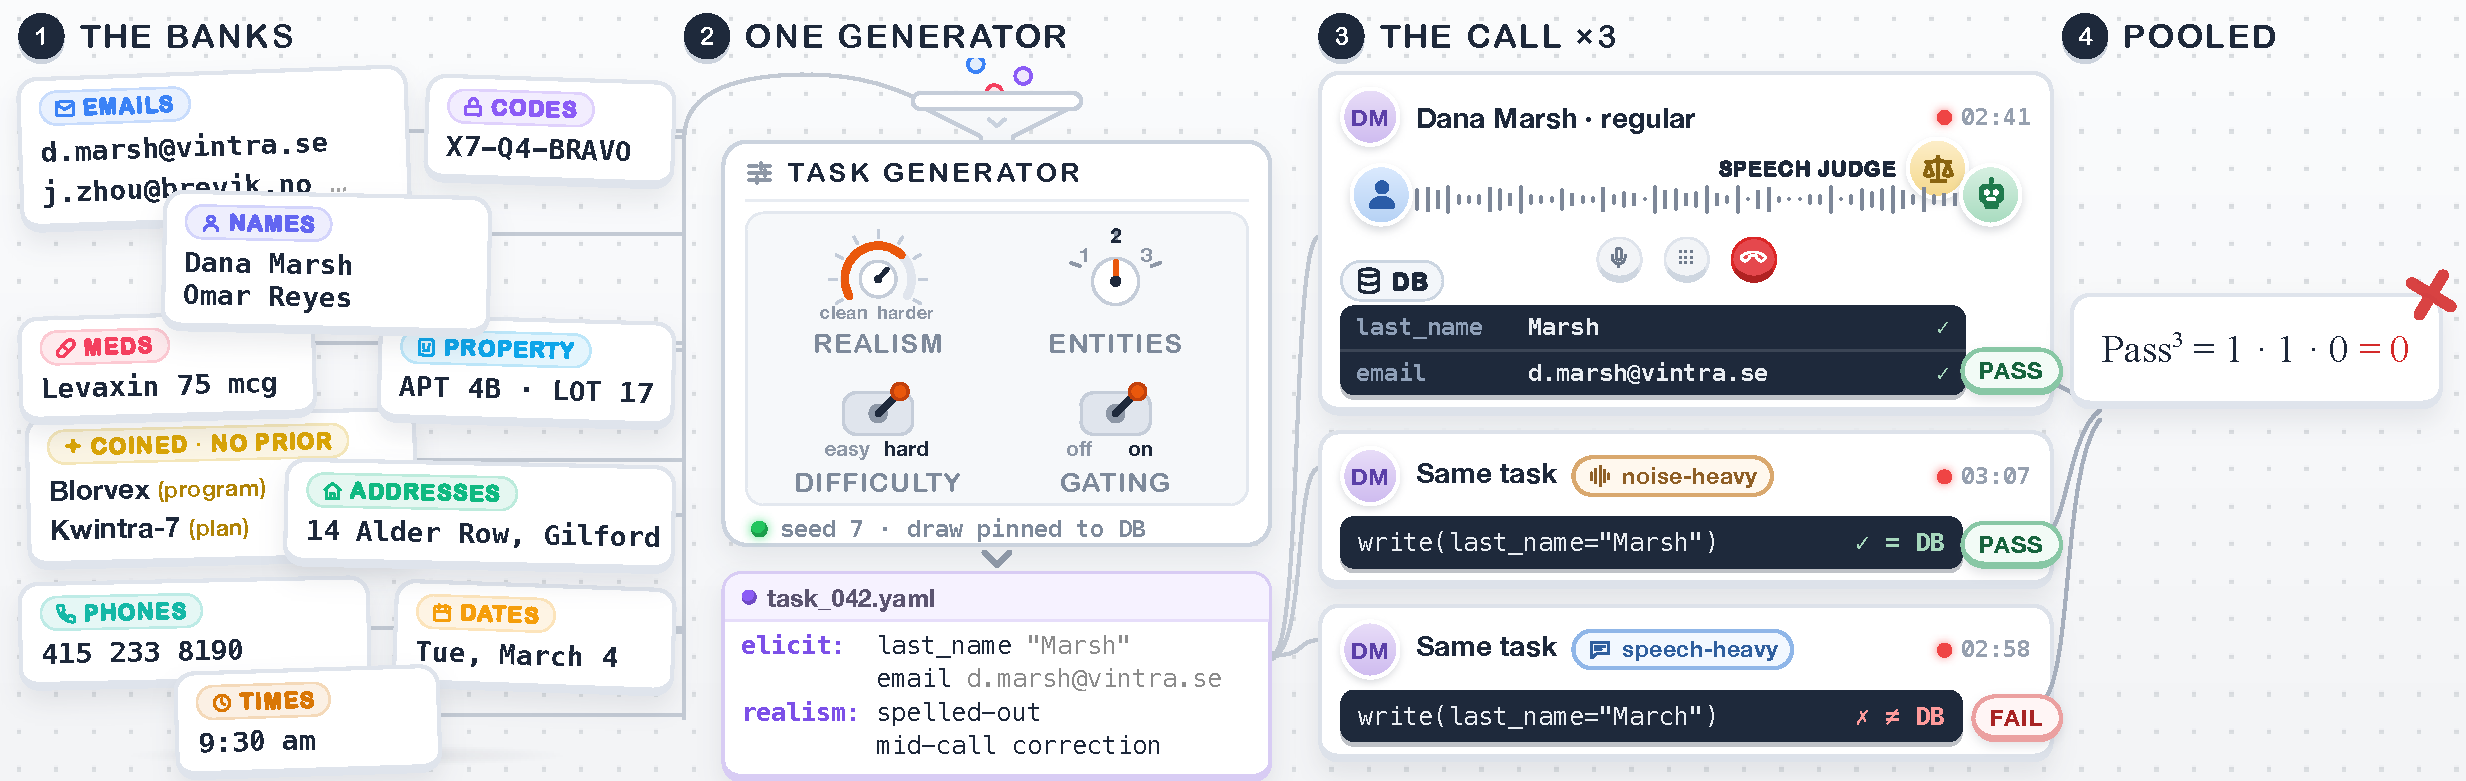
\includegraphics[width=\textwidth]{figures/task_generator_pipeline.pdf}
\caption{\telicit{} selects values from entity banks, builds a controlled task,
and runs it through the \tauvoice{} interaction loop. \passk{} requires success
in all three environment realizations. The scale marks fidelity-judged agent
speech.}
\label{fig:pipeline}
\end{figure*}

\section{Related Work}
\label{sec:related-work}

\begin{table}[t]
\caption{Coverage of related benchmarks. \edited{Multi: multi-turn}; Task: executed tool task; Exact: exact entity score;
$N$: controlled entity count; D: diagnostic or partial coverage.}
\vspace{3pt}
\label{tab:related}
\centering
\small
\setlength{\tabcolsep}{2pt}
\renewcommand{\arraystretch}{.9}
\begin{tabular}{@{}lccccc@{}}
\toprule
Work & Multi & Task & Exact & $N$ & Repair \\
\midrule
Voice agents \cite{ray2026tauvoice,bogavelli2026evabench,bhosale2026duplexworld,lin2026fdbv3} & $\checkmark$ & $\checkmark$ & D & -- & D \\
Spoken dialogue \cite{si2023spokenwoz,zhang2022slot} & $\checkmark$ & -- & $\checkmark$ & -- & -- \\
Speech NER \cite{shon2022slue,yu2024heard,assemblyai2026mer} & -- & -- & $\checkmark$ & -- & -- \\
\telicit{} & $\checkmark$ & $\checkmark$ & $\checkmark$ & $\checkmark$ & $\checkmark$ \\
\bottomrule
\end{tabular}
\end{table}

Existing voice-agent benchmarks---\tauvoice{}, EVA-Bench, DuplexWorld, and
Full-Duplex-Bench-v3---measure end-to-end task performance and interaction
quality; several also exercise tool use
\cite{ray2026tauvoice,bogavelli2026evabench,bhosale2026duplexworld,lin2026fdbv3}.
Their broad scope reveals failures such as authentication---identified as the
dominant bottleneck in \tauvoice{} and reported separately in EVA-Bench---but
does not isolate exact entity capture
\cite{ray2026tauvoice,bogavelli2026evabench}. \telicit{} extends the
\mbox{$\uptau$-bench}, \mbox{$\uptau^2$-Bench}, and \tauvoice{} lineage by making
controlled voice entity collection the primary task
\cite{yao2024taubench,barres2025tau2bench,ray2026tauvoice}.

Dialogue-state tracking spans MultiWOZ, SpokenWOZ, and cross-utterance sub-slot
tracking
\cite{budzianowski2018multiwoz,si2023spokenwoz,zhang2022slot}.
ASR and spoken-entity work covers natural-speech NER, ASR error propagation,
unseen entities in synthesized audio, and industrial missed-entity rates
\cite{shon2022slue,szymanski2023ner,yu2024heard,assemblyai2026mer}.
\emph{Error Detection and Recovery in Spoken Dialogue Systems} studies repair strategies
\cite{filisko-seneff-2004-error}. None combines live tool execution, exact
database writes, controlled entity type, difficulty and count, \edited{and} an agent's
choice to verify. Table~\ref{tab:related} summarizes this gap.

\section{Methods}
\label{sec:methods}

\subsection{Task and elicitation policy}
\label{sec:elicitation-policy}

Each task is a callback about a record with missing fields. The agent sees the
field names, asks the caller for their values, logs its captures, and submits
once; the caller reveals a value only after it is requested. The simulated
caller is cooperative: it supplies requested values, spells accurately when
asked, and confirms or corrects read-backs, but never volunteers information.

\subsection{Values, difficulty, and realisms}

Ten banks each contain 40 easy and 40 hard values; the benchmark samples 10 of
each difficulty per bank. Difficulty is type-relative: for example, hard names
are rarer, hard codes are longer or confusable, and hard emails contain more
symbols. Table~\ref{tab:entity-results} reports bank construction and
performance.

A seeded catalog adds six caller realisms by appending a scripted instruction
to the caller prompt. For example, one spelling-style instruction tells the
caller to say ``zed'' for the letter Z whenever spelling a value.
Self-correction supplies a wrong value and immediately repairs it; spelling
variation changes how letters or digits are grouped; falter-and-restart
spelling introduces a mid-string correction; partial and wrong-field answers
require a follow-up; and reviewed mispronunciations alter only the audio.
Conditional behaviors occur only when the conversation creates an opportunity,
so a spelling correction, for example, cannot fire until spelling begins. Each
task stores its generator and catalog versions, seed, selected realism, and
expected database state. The generator also emits linked two- and three-field
tasks, both as flat calls and as a staged workflow that validates one field
before revealing the next.

\subsection{Scoring and behavioral measures}

\edited{Exact success requires database equality after type-specific
normalization (e.g., phone-number separators). We report}
regular-realization success as \passone{}. We define robust \passk{} as exact
success on the same task across three prespecified environment realizations:
\emph{regular};
\emph{noise-heavy}, with 10\,dB background noise, bursts, frame drops, and
muffling; and \emph{speech-heavy}, with interruptions, backchannels, and
restarts. Unlike a repeated-trial score, \passk{} crosses these prespecified
conditions; voices and realism assignments are also redrawn. A 700-call audit placed the 90th-percentile duration at 1.89
minutes, so we use a conservative four-minute limit. Timed-out calls remain in
the denominator and score zero.

\corrected{Post-hoc review found a unit-normalization mismatch. The evaluator
now normalizes ``milligram(s)'' to ``mg''.}

\edited{Behavioral analysis compares first and submitted values with gold
after case/punctuation folding.} Silent caller tools log every spelling request and read-back; their
sum is our measure of verification effort. We compare this effort across noise,
entity difficulty and familiarity, and each system's best- and worst-performing
caller voices.

\section{Experiments}
\label{sec:experiments}

We evaluate gpt-realtime-2 (minimal and xhigh reasoning),
gemini-3.1-flash-live-preview (high), and grok-voice-think-fast-1.0
(provider default)
\cite{openai2026models,google2026models,xai2026grokvoicethinkfast}.
The caller uses gpt-5.5 (xhigh, temperature zero) \cite{openai2026models},
with speech synthesized by ElevenLabs eleven\_v3
\cite{elevenlabs2026elevenv3}.

\edited{We compare agent-directed and scaffolded prompting on the same tasks.}
Each configuration runs all 200 tasks under the regular, noise-heavy, and
speech-heavy conditions \edited{with each prompt}. This gives 600 agent-directed and 600
scaffolded calls per configuration, or 4,800 calls in total.
\edited{Behavioral, caller-voice, and bank-level analyses use three
configurations: GPT xhigh, Gemini high, and Grok.}

\edited{Main-run confidence intervals} come from 10,000 task-level bootstrap samples. When a task
is sampled, its three linked conditions stay together. Pairwise system tests
also align calls by task. We use a two-sided sign-permutation test with 100,000
permutations and the standard $+1$ correction. Holm correction is applied
separately to the six system comparisons for \passone{} and \passk{}.

Two raters independently review 90 \corrected{reward-zero} calls across providers, labeling
failure source and subtype. After discussion and \corrected{nine} explicit adjudications,
failure source is resolved for 86 of 90 calls and subtype for 66 of the 81
calls resolved as agent failures.
For fidelity validation, gemini-3.1-pro-preview (temperature zero) scores a
frozen stratified 60-utterance sample enriched for human flags
\edited{(30 Gemini and 30 Grok utterances)}
\cite{google2026models}.

\section{Results}
\label{sec:results}

\begin{figure}[t]
\centering
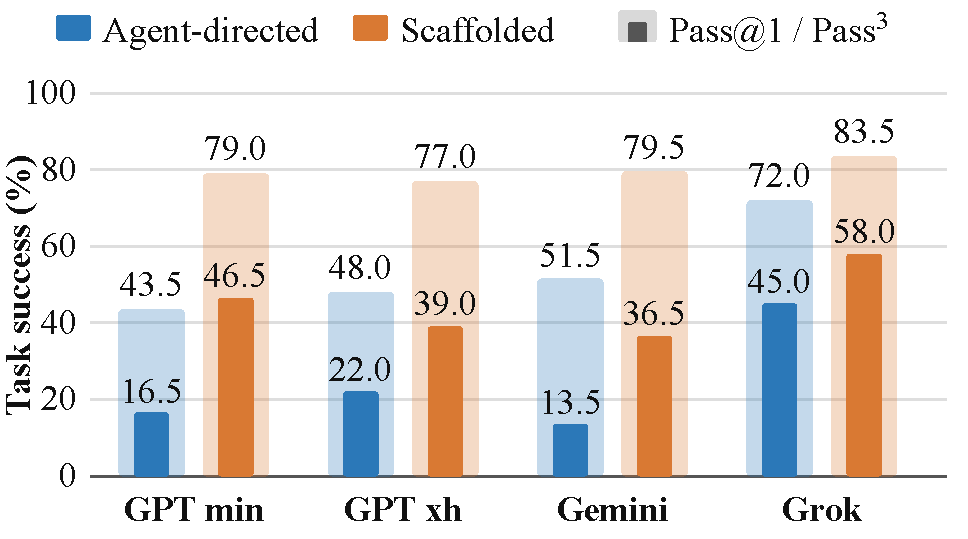
\includegraphics[width=\columnwidth]{figures/accuracy_effort_dumbbell.pdf}
\caption{Task success over \edited{200 single-field tasks for four configurations}.
Each pair shows
agent-directed and scaffolded runs; light full bars show \passone{},
and dark inset bars show robust \passk{}.}
\label{fig:main-results}
\end{figure}

\subsection{Strategy selection and robustness}

\begin{list}{\textbullet}{
\setlength{\leftmargin}{1.15em}
\setlength{\labelwidth}{0.45em}
\setlength{\labelsep}{0.35em}
\setlength{\itemsep}{0pt}
\setlength{\parsep}{0pt}
\setlength{\parskip}{0pt}
\setlength{\topsep}{0pt}
}
\item \textit{Scaffolding trades time for reliability.} \edited{Scaffolded runs
score \corrected{12--36} points higher on \passone{} and \corrected{13--30} points higher on \passk{}}
(Figure~\ref{fig:main-results}), \edited{with 21--28 additional seconds per call
across the three behavioral configurations}. Gains are
slightly larger for hard entities (\corrected{25 versus 21 points}).
\item \textit{A supplied protocol narrows provider gaps.} Grok remains best
and significantly exceeds every other agent-directed system on both measures
(\corrected{Holm-adjusted $p<.001$}); \edited{no other pair is significant}.
\edited{The comparison suggests that explicit verification instructions improve reliability.}
\item \textit{Robustness exposes instability.} Across systems, \passk{} spans
\corrected{14--45\% agent-directed and 37--58\% scaffolded}. Rankings can reverse: Gemini
beats GPT xhigh on regular \passone{} (51.5\% versus \corrected{48.0\%}), yet trails on
\passk{} (13.5\% versus \corrected{22.0\%}).
\item \textit{Diverse environments expose more than run-to-run variation.}
For scaffolded GPT xhigh, three regular runs have similar \passone{} rates
(74.5\%, 75.5\%, and 77.0\%), yet only 103 of 200 tasks pass
every repeat (\passk{} = 51.5\%): 86 tasks change outcome at least once.
Replacing two repeats with noise-heavy and speech-heavy conditions lowers the
all-three count to \corrected{78 (39.0\%)}.
\edited{The crossed conditions expose additional instability in this comparison.}
\item \parbox[t]{\linewidth}{\textit{More reasoning does not consistently
improve robustness.} From minimal to xhigh, \passk{} rises from
\corrected{16.5\% to 22.0\%} agent-directed but falls from
\corrected{46.5\% to 39.0\%} scaffolded.}
\end{list}

\subsection{Risk recognition and recovery}

\edited{In regular agent-directed calls, wrong first captures are logged for
\corrected{134/200} GPT xhigh fields, 129/199 Gemini fields, and
\corrected{74/193} Grok fields
(\corrected{67/65/38\%}); 7/22/14 fields have no capture log.}
GPT and Gemini verify 66\% and 64\% of wrong captures
versus \corrected{49\% and 50\%} of correct ones; Grok verifies nearly everything
(\corrected{93\%/96\%}). The
systems likewise spend more effort on hard and unfamiliar entities;
\corrected{GPT xhigh and Grok, but not Gemini, spend more on their
lowest-performing caller voice}, and only Grok reacts to noise
(Figure~\ref{fig:adaptivity-effort}). \edited{Verification is selective but imperfect.}

\begin{figure}[t]
\centering
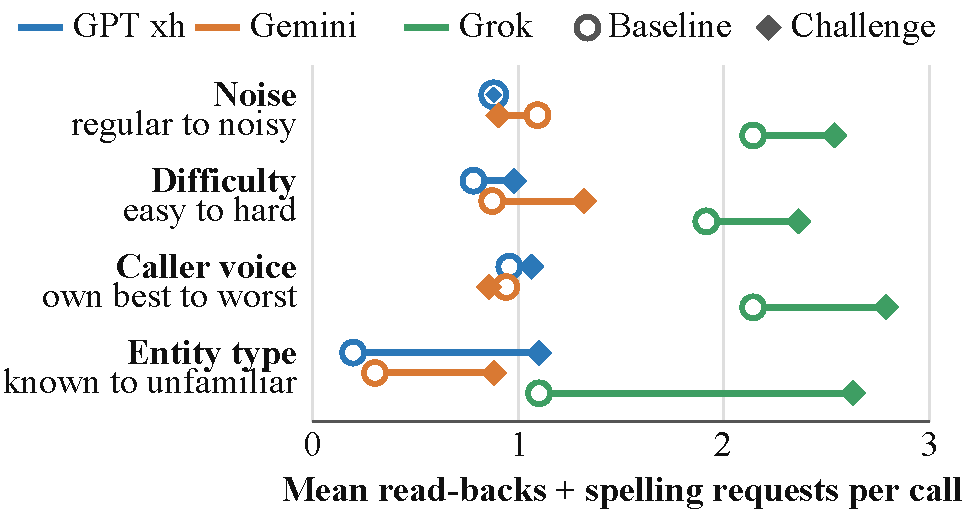
\includegraphics[width=\columnwidth]{figures/adaptivity_effort.pdf}
\caption{Mean verification effort (read-backs plus spelling requests). \edited{The three}
systems increase effort for hard and unfamiliar entities. \corrected{GPT xhigh
and Grok, but not Gemini, increase it for their own lowest-\passone{} caller
voice}; only Grok increases effort under noise.}
\label{fig:adaptivity-effort}
\end{figure}

Only \corrected{30\%, 37\%, and 32\%} of verified GPT xhigh, Gemini, and Grok errors end
correct. Among \corrected{337} initially wrong captures, recovery is 10\% without a repair
step, \corrected{31\%} with read-back only, 24\% with spelling only, and
\corrected{39\%} with both.
Because agents choose when to verify, these are associations, but the pattern
\edited{suggests a recovery bottleneck even when verification occurs}. Agents \edited{can} double down on an
error or hallucinate a replacement rather than complete the repair.

Caller voice is another blind spot. In agent-directed regular calls, the gap
between each system's best- and worst-performing voices is \corrected{26 points} for GPT
xhigh, 28 for Gemini, and \corrected{12 for Grok}. The ordering is not stable: Mildred leads
GPT xhigh and Grok, whereas Wei leads Gemini. Only Gemini shows evidence that
success differs across all five voices after correction ($p=.040$); no
individual Gemini voice pair remains significant, so the result establishes
heterogeneity without isolating one contrast. Across systems, Mildred
significantly exceeds \corrected{Mamadou and Arjun, but not Priya or Wei}.
\corrected{GPT xhigh and Grok increase verification effort for their weakest
voice; Gemini does not.}

\subsection{Stress tests and diagnostics}

\edited{Caller realisms show clearer effects on repair cost than success.} No assigned realism
detectably changes exact success in either arm (Figure~\ref{fig:realism-effects}).
Overall H\'ajek estimates are \corrected{$-2.1$ points (95\% CI $[-8.6,4.3]$)}
agent-directed and \corrected{$-4.2$ ($[-8.8,0.4]$)} scaffolded. Assigned realisms may
remain latent. In agent-directed runs, \edited{the mispronunciation success
estimate is \corrected{$-3.0$ points}, while the probability of a spelling request is
24 percentage points higher and calls are 26 seconds longer. These null
success tests do not establish absence of an effect.}

\begin{figure}[t]
\centering
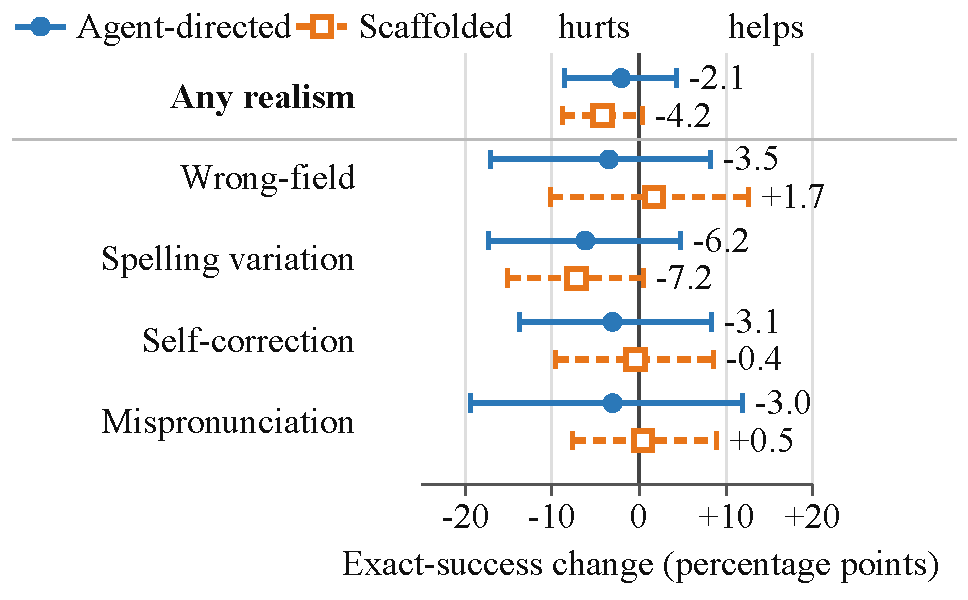
\includegraphics[width=\columnwidth]{figures/realism_assignment_effects.pdf}
\vspace{-22pt}
\caption{Caller-realism effects in agent-directed (solid circles) and
scaffolded (dashed squares) runs. Bars show task-clustered 95\% H\'ajek
intervals versus eligible clean assignments; none survives Holm correction.}
\label{fig:realism-effects}
\end{figure}

\begin{table}[t]
\caption{Value-bank construction and robust agent-directed results. Every bank
has 80 values and contributes 20 tasks (10 easy, 10 hard).}
\vspace{3pt}
\label{tab:entity-results}
\centering
\small
\setlength{\tabcolsep}{2pt}
\renewcommand{\arraystretch}{.9}
\begin{tabular}{@{}>{\raggedright\arraybackslash}p{.25\columnwidth}
                    >{\raggedright\arraybackslash}p{.52\columnwidth}c@{}}
\toprule
Bank & Construction / grounding & \passk{} \edited{(desc)} \\
\midrule
Dates        & Calendar and clock & .60 \\
Phones       & Regulator-reserved ranges & .47 \\
Times        & Calendar and clock & .43 \\
Person names & SSA + Census \cite{ssaNames,censusSurnames} & .30 \\
Codes        & ISO 3779 VINs; mod-97 IDs & .25 \\
Medications  & RxNorm-checked \cite{nelson2011rxnorm} & \corrected{.23} \\
Properties   & Registry-screened synthetic & .18 \\
Addresses    & Synthetic address grammar & .10 \\
Emails       & DNS-nonresolving domains & .08 \\
Coined       & Registry-screened synthetic & .03 \\
\bottomrule
\end{tabular}
\end{table}

\edited{Performance varies by entity type.} Across the regular
agent-directed cells, \passone{} is \corrected{67.0\%} on easy entities and
\corrected{47.3\%} on hard
ones; scaffolding raises these rates to \corrected{87.7\% and 72.3\%}. Pooled \passk{}
ranges from \corrected{3.3\% for coined names} to 46.7\% for
phone numbers and 60.0\% for dates (Table~\ref{tab:entity-results}). The pattern
is consistent with format-constrained versus lexical capture. Dates and phone
numbers follow tightly scoped numeric schemas. \corrected{Medications reach 23.3\%
after unit normalization and} come from a closed
RxNorm vocabulary and coined names from a synthetic registry, but the agent is
shown neither list.

\begin{table}[t]
\caption{\edited{Field validation and retry comparison: GPT xhigh,
90 multi-field tasks $\times$ three trials per arm; $\pm$ gives 95\% Wald
margins}. Task
\passone{} requires every field to be correct; field \passone{} scores
individual values.}
\vspace{3pt}
\label{tab:protocol-ablation}
\centering
\small
\setlength{\tabcolsep}{4pt}
\renewcommand{\arraystretch}{.9}
\begin{tabular}{@{}>{\raggedright\arraybackslash}p{.51\columnwidth}cc@{}}
\toprule
Workflow & Task \passone{} & Field \passone{} \\
\midrule
Batch submit; no field validation & $.64\pm.06$ & $.78\pm.03$ \\
Validate each field; retry errors & $.82\pm.05$ & $.86\pm.03$ \\
\bottomrule
\end{tabular}
\end{table}

\begin{figure}[t]
\centering
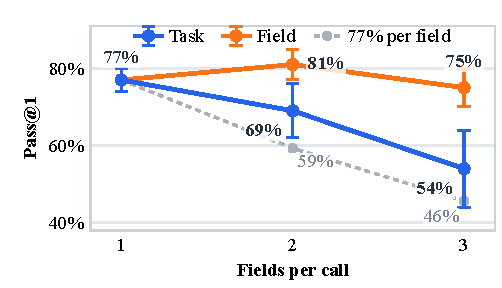
\includegraphics[width=\columnwidth]{figures/composition_results.pdf}
\vspace{-16pt}
\caption{\edited{Scaffolded GPT xhigh ($n=630/180/90$ observations for
one/two/three fields). The gray reference assumes independent 77\% success
per field. Bars show approximate 95\% Wald intervals, not adjusted for repeated
tasks; the single-field reference reuses matched calls.}}
\label{fig:composition-results}
\end{figure}

\edited{Errors compound across fields.} At three fields, only \corrected{54\%} of
calls pass even though individual fields remain \edited{75\%} accurate
(Figure~\ref{fig:composition-results}): one wrong field fails the entire call.
Intermediate validation and retry counter this accumulation, raising task
accuracy from \edited{64\% to 82\%} across the \edited{same} multi-field tasks
(Table~\ref{tab:protocol-ablation}). Because the intervention combines both
mechanisms, we do not attribute the gain to either one alone.

\begin{table}[!ht]
\caption{\edited{Regular agent-directed utterances} with a clear speech-fidelity defect
by system (lower is better). \edited{Scored $n$: 945, 1,142, 1,046, and 1,813,
respectively.}}
\vspace{3pt}
\label{tab:fidelity-provider}
\centering
\small
\setlength{\tabcolsep}{3pt}
\renewcommand{\arraystretch}{.9}
\begin{tabular}{@{}lcccc@{}}
\toprule
& GPT minimal & GPT xhigh & Gemini high & Grok \\
\midrule
Severity $\geq 2$ & 2.5\% & 2.1\% & 3.6\% & 4.1\% \\
\bottomrule
\end{tabular}
\end{table}

\corrected{Human review of 90 original reward-zero calls attributes 81 to the
agent, one to user-simulator logic, four to infrastructure scoring errors, and
leaves four unresolved; reported scores use the corrected grading.} Among the 81 agent
failures, agreed or adjudicated labels assign 42 as transcription, 16 as
logical, six as VAD, and two as hallucination; the remaining 15 retain subtype
disagreement. The speech-fidelity judge
compares agent audio with its reference transcript, flagging mispronunciations,
word additions, omissions, and clipping; severity $\geq 2$ marks a clear,
potentially confusing mismatch \edited{(Table~\ref{tab:fidelity-provider};
findings overlapping the final second are excluded to prevent truncation false
positives)}. \edited{The 60-utterance set} yields .80 precision, .75
recall, and .77 F1. \edited{A separate GPT-5.5 xhigh text control passes all
200 tasks with the scaffolded policy, showing that the task set is
straightforward for a capable text model.}

\section{Conclusion}

Voice agents still struggle to collect exact entities reliably. Our caller is
deliberately highly cooperative: it spells accurately and corrects faulty
read-backs. Even under these favorable conditions, \edited{agent-directed
systems achieve robust \passk{} on only \corrected{14--45\%} of tasks, compared with
\corrected{37--58\%} with scaffolding}.

\vspace{3pt}
\noindent Failures occur at both stages of recovery: agents do not consistently
recognize risky captures, and when they do verify an error, only
\corrected{30--37\%} are repaired.

\subsection*{Limitations}
We study English, three providers, one simulator,
and one run per main environment. We intentionally omit caller-side ASR to
avoid confounding agent performance with a second recognizer. As a result,
agent speech synthesis is not evaluated end to end: the speech-fidelity judge
reports synthesis defects, but they do not yet affect task reward. The
multi-field study is formative; broader provider, human-caller, and
multilingual validation remain future work. \edited{Human validation of the
fidelity judge covers Gemini and Grok only.}

\section*{ACKNOWLEDGMENT}
We thank Ben Shi, Ola Zytek, Vijay Iyengar,
Ajeet Grewal, and Clay Bavor for feedback and support.
\edited{OpenAI Codex and Anthropic Claude Code assisted, under author review,
with manuscript drafting/editing and benchmark, analysis, and figure code.}

\clearpage

\section{Compliance with Ethical Standards}

The benchmark uses no real customer records or recordings. Values are
synthetic or public and non-sensitive; calls use simulated callers and provider
voices. Reviewers consented and were compensated.

Exact-value elicitation is dual use: it can improve service calls but can also
facilitate collection of sensitive identifiers. Deployments should minimize
collection, explain its purpose, protect stored values, and support human
escalation. Our simulated English results are not evidence of safety, privacy,
deployment readiness, or differences among people or demographic groups.

This work was supported by Sierra and Mercor. The authors are employees of
Sierra and Mercor, respectively, and have no other relevant interests to
disclose.

\raggedcolsend
\bibliographystyle{IEEEbib}
\bibliography{references}

\end{document}
